% Selector (Fallback) composite with textbook-style leaves.
\documentclass[border=6pt,tikz]{standalone}
\usepackage{tikz}
\usepackage{amsmath, amssymb}
\usepackage[T1]{fontenc}
\usepackage{lmodern}
\usetikzlibrary{arrows.meta, positioning, shapes.geometric}

\tikzset{
  composite/.style = {draw, rounded corners=2pt, fill=blue!10, align=center,
                      font=\small\bfseries, inner sep=4pt,
                      minimum width=1.8cm, minimum height=0.8cm},
  condition/.style = {draw, ellipse, fill=yellow!18, align=center,
                      font=\scriptsize, inner sep=3pt,
                      minimum width=1.35cm, minimum height=0.7cm},
  action/.style    = {draw, rectangle, fill=green!16, align=center,
                      font=\scriptsize, inner sep=3pt,
                      minimum width=1.35cm, minimum height=0.7cm},
  flow/.style      = {-, line width=0.55pt},
}

\begin{document}
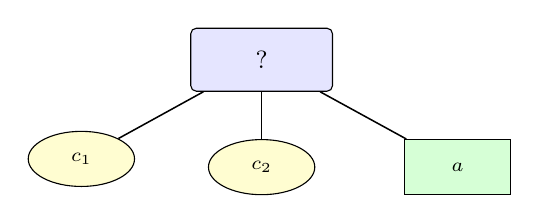
\begin{tikzpicture}[node distance=0.6cm and 0.9cm]
  \node[composite]                   (r) {$?$};
  \node[condition, below left=of r]  (a) {$c_1$};
  \node[condition, below=of r]       (b) {$c_2$};
  \node[action,    below right=of r] (c) {$a$};
  \draw[flow] (r) -- (a);
  \draw[flow] (r) -- (b);
  \draw[flow] (r) -- (c);
\end{tikzpicture}
\end{document}
